\section{Overview}
% \subsection{Introduction of overall field and basic explaination of this topic (What)}
% I) Opening Section
%   1) Introduce the overall field 
% Aircraft noise is one of the most environmentally detrimental consequences of
% commercial flight. Studies suggest that exposure to aircraft noise leads
% to dimished academic performance in youth, and could increase the risk of 
% cardiovascular disease for populations close to airports \cite{Basner2017}. 
% Although the COVID-19 pandemic reduced air panssenger trafic by 96\% between 2019 
% and 2020, \cite{pandemicReport} the global aviation commmunity has proven 
% to be resilliant during times of economic shock. The International Air Transport
% Association (IATA) has studied the resilience of the global air passenger markets after four notable shocks to the aviation economy; 
% The impact of four notable events, (1979 oil shock, 2000-2001 dot-com bust, 9/11, and the 2008 financial crisis) 
% was studied by a statistical analysis of the estimated 'passenger gap' from 1950-2014. 
% Data shows that approximately 72\% of the impact of the initial shock persists 
% one year after the event and diminishes to just under one-fifth of the initial impact. 
% Given these trends in air transportation, the need for  aviation noise  
% regulation persists and will continue to be a concern so long as the aviation
% continues this rate of growth.

% II) Background and overview
%      What is the current situation with aircraft noise
%      wht are acoustic modes and liners
%      Swirling flow codes
%      code verification
%   1) What is sound propagation and why is it relevant in ducted flows? 
%   2) What are the key theories and research
%   3) what is the current context and what does this mean
Since the dawn of commerical airlines in the early 20th centurty, the increased demand for aircraft transport
introduced jet engines to support large cargo and passengers. Consequently,
this rise in innovation resulted in high volume engine noise due to 
the frequency of flights. After 1975, 
efforts to reduce aircraft noise eliminated the noise pollution for 90\% of
the population \cite{FAAPolicy}.  However, given the rapid increase in
aircraft movements and consequently increase in noise exposure to larger 
populations, the advancement in noise reduction 
technologies has only been moderately increasing, leaving a requirement for 
in aeroacoustic modeling techniques and treatment strategies to compete with 
the demand for quiet subsonic flight \cite{icao2020}.  
%   2) Introduce the research problem
% The 
Between the 1950s and 1960's jet engine designs shifted to higher by pass 
ratios with two or three shafts. The high by pass ratio (HBP) fan utilized multiple
stages of fans and  air streams \cite{smith1989aircraft}. The efficiency of these
engines rose with the availablility of materials that are able to cool flows
passing over the turbofan, thus slowing the overall jet velocity but maintaining the 
efficiency of the engine. 
% One of the most popular configurations is the geared 
% turbofan (GTF), the largest contributor to the noise on modern aircraft 
% has been the fan upon take-off and landing.  Although the use of the GTF has
% reduced the noise emissions by 75\% \cite{GTFinfo}, further noise reduction
% technologies to mitigate the noise associated to the turbofans geometric
% configuration and operation speeds. One of the most common techiques to reduce 
% fan noise  is to include the use of acoustic treatment along the walls of the
% turbomachine's nacelle. 
Due to the increase in high-bypass-ratio of turbomachines, the newest models of 
engines have a significantly larger diameter and a shorter nacelle, leaving less
room to place acoustic treatments in regions where it will be effective \cite{Kozaczuk2017}.
Figure \ref{fig:intro} shows the evolution of directivity for turbomachines as 
the use of HBR fans became more popular. As these engines continue 
to develop, an increased understanding of sound propagation within
the interstage of the engine is gong to be needed due to flow behavior (high compressibility
and rotational effects).  While a turbomachine's general flow condition includes 
a series of axial, tangential, and radial velocity components that vary
depending on the location of concern, the swirling flow between fan stages has 
been an area of interest due to the potential for acoustic treatment in a 
location previously avoided for its flow complexity. This work will explore how 
sound propagation is modeled and how the current state of code verification and 
validation (V\&V) currently stands. This introduction will describe how fluid mechanics
is utlized to establish an aeroacoustic model for various ducted flows. It will 
also discuss how code verification is used in the computational and numerical fields
but will show the need for the use of these code verification techniques for 
a frequency domain CAA code. 


%   3) State your research aims

%   4) Outline the introduction 

%3)
\begin{figure}
    \centering
    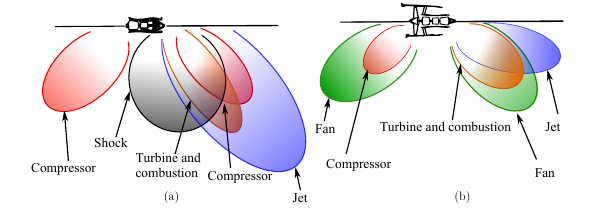
\includegraphics[width=\textwidth]{Chapter-1-Introduction/Figures/lowVhighBPRdirectivitySMITH2004.png}
    \caption{ The evolution of the directivity and the 
    relative levels of sources as a function of engine architecture (a)low bypass-ratio (b) high bypass ratio \cite{smith1989aircraft}}
    \label{fig:intro}
\end{figure}

% \section{Statement of the of the research questions}
% \subsection{What is already known?}
% III) Research Problem

%   1) What's already known?
%   2) What's missing?
%   3) Why is it a problem?
In general, jet engine designers can model flow within a turbomachine with 
the Navier Stokes (N-S) Equations, a set of partial differential equations that
describe the mass, momentum and energy of a given viscous fluid, however 
these equations can be computationally expensive as they are used in the most
general cases. 

For aeroacousticians, the N-S equations can be  
to identify sound generation and propagation because acoustic waves are low 
amplitude (~ only a fraction of atmospheric pressure) and are not strongly
influenced by viscosity.   

As a result, it is common in practice to 
utilize the Linearized Euler equations (LEE),
a closely related set of PDEs that model inviscid fluid, as they provide an 
approximation for higher Reynold number flows where viscosity 
does not play a critical role. ach to modeling sound propagation 
within a flow is to ``linearize'' the Euler equations, which decomposes the 
flow solution into a mean and fluctuating component . The decomposition is done 
in a linear fashion because the sound propagation amplitude is small with respect
to the mean flow, and their presence does not appreciable change the mean flow 
field. The flow solution\'s decomposition gives rise to linear and nonlinear terms 
in the Euler equations where the non-linear fluctuating components are neglected. 

The LEE provides a system of linear equations where the solution is a family of wavenumbers and radial mode shapes that arise from 
unsteady disturbances for flows within a cylindrical duct.  Another method 
decomposes the flow into vortical and potential parts \cite{golubev1996sound}.
In either case, this presents an initial value problem which 
in limited cases can obtain analytical solutions for simplified mean flow. Once a mean flow 
is contains a tangential component, the LEE equations must be solved numerically.  
% \subsection{What is missing?/Why is it a problem?}
For uniform flows in a hard wall duct , the waves are categorized as vortical 
,entropical, and acoustic waves. The vortical and entropic waves soley convect with 
the mean flow, where as the acoustic wave can propagate without damping or decay 
exponentially.  However, for swiriling flows, the waves are partially coupled
and are not easily categorized due to an additonal category of ``nearly convecting'' 
modes \cite{Kerrebrock2012},\cite{KERREBROCK1974} . 
Therefore, the families of waves must be found numerically \cite{Envia2004}
making the ducted acoustic propagtion in swirling flow a problem without
an analytical solution but has a framework for a numerical solution.
% \subsection{The goal and significance of the investigation}
Swirling flow has been a difficult problem to investigate in comparison to 
flows parallel to the wall domain of a duct \cite{COOPER2001} because of the 
lack of an analytical solution and thus cannot be described from a single convective 
wave equation. However, the solution for sheared mean flows was first presented
by Goldstein \cite{Goldstein1978},\cite{Goldstein1979}. Various special cases of
swirling flow (free vortex and solid body swirl) was examined in \cite{KAPUR1973}
\cite{Kerrebrock2012}, \cite{KERREBROCK1974}. In recent years V \& V has been 
done given the rise in technologies capabale of experimentally
measuring the acoustic modes within a turbomachine \cite{Maldonado2016}. This
work aims offer additional insight to the V \& V process 
by expanding on techniques used in this field.  

Computational codes are widely used in the field of aeroacoustics and concerted
effort has recently been made to improve V \& V techniques 
by Ingraham and Hixon \cite{Ingraham2015,Ingraham2010}. The question of getting 
the correct answer was a large focus of this work. 

This thesis aims to continue this effort by conducting code verification and validation on a frequncy domain 
Linearized Euler equation approximation on previous work done by Pratt \& Whitney
and NASA Glenn Research Center though techical contract \cite{kousen1996pressure,kousen1995eigenmode}.  

% \section{Definition of the terms (if needed)}
% define verification and validationr

The algorithms presented in this thesis have been written using FORTRAN 77 and 
has been updated to FORTRAN 90, and implemented into a code named SWIRL. The 
foundational work has been started by Pratt and Whitney by Kenneth Kousen 
\cite{kousen1996pressure} and continuted by Dr. Ray Hixon. SWIRL analyzes 
axial flows with mean shear and swirl in hard wall and acoustically lines ducts.
The Method of Manufactured Solutions (MMS) is a process for generating an 
analytical solution for a code that provides the numerical solution for a 
given domain. The goal of MMS is to establish a manufactured solution that can 
be used to establish the accuracy of the code within question. For this study, 
SWIRL, a code used to calculate the radial modes within an infinitely long duct
is being validated through code verification. SWIRL accepts a given mean flow and 
uses numerical integration to obtain the speed of sound. The integration technique
is found to be the composite trapezoidal rule through asymptotic error analysis.

Prior work has largly depended on conducting code validation through exact solutions
to the partial differential equation (PDE) , the convective wave equation . Such a
procedure formally known as the method of exact solutions (MES) \cite{MESref}. 
MES has the advantage in that the output of SWIRL can be directly compared 
to the solution of the PDE, however available solutions are limited for sound
propagation in ducted flows.


    
% \section{Organization of research (Structure)}
% IV) Research aims, objectives, and research question
% V) State benefit/significance
% - speed improvement 
% VI)
% VII)


The literature review in the next chapter will discuss the governing equations that are
used to predict the acoustic behavior in a fluid flowing internally, followed 
by the research problem that arises in swirling flow, the objectives and 
questions, the significance and finally the limitations.  The proposed research aims to determine the impact of the numerical schemes used
in the swirling flow problem and how it effects the family of waves that are
produced from the problem formulation so a better understanding of the 
acoustic phenomena as the flow under goes a compressible rotational flow. The use
of the method of manufactured solutions is used as a means of ensuring the code is
correctly approximating the goverining equations and will check the effect of the numerical schemes
on the axial wavenumbers produced.
 
% \section{Research Questions and Hypothesis}

The use of numerical approximations are powerful for cases where 
there is no analytical solution, thus leaving multiple ways of arriving at a
numerical solution. The use of MMS allows the user to obtain various metrics
such as the approximated asymptotic rate of convergence, or the grid convergence index,
to identify if the code is performing as intended , i.e. using the right equations.


The goal of this research is to conduct component level code verification tests 
for the problem of characterizing the duct acoustics for flow using a LEE model 
by looking at the two numerical components for SWIRL.


The goal o
The proposed component verification from Kleb and Wood will 
be presented to addreess the characterization of 
modes and the presence of numerical ones. 

Hypothesis.
further improve the result. 


